\chapter{Aprendizado de Máquina}


AM pode ser altamente benéfico para solução de problemas complexos, é possível observar um ciclo de trabalho bem definido que está presente na solução de problemas por uma abordagem de Aprendizado de Máquina. As etapas gerais de projetos de AM são aquisição de dados, construção de modelo, análise, otimização e predição \cite{real2013}. Com estas cinco etapas é possível sair de um conjunto de dados e chegar as respostas desejadas através de cuidadosa seleção e processamento de dados, passando pela construção e avaliação de um método eficaz até chegar a um modelo consistente com a necessidade do problema. Embora haja uma linearidade na execução desses processos é comum em projetos de AM revisitar estas etapas várias vezes. A imagem a seguir revela um ciclo de AM mais detalhado e que engloba as etapas previamente citadas ressaltando elementos importantes: 

\begin{figure}[!h]
\centering
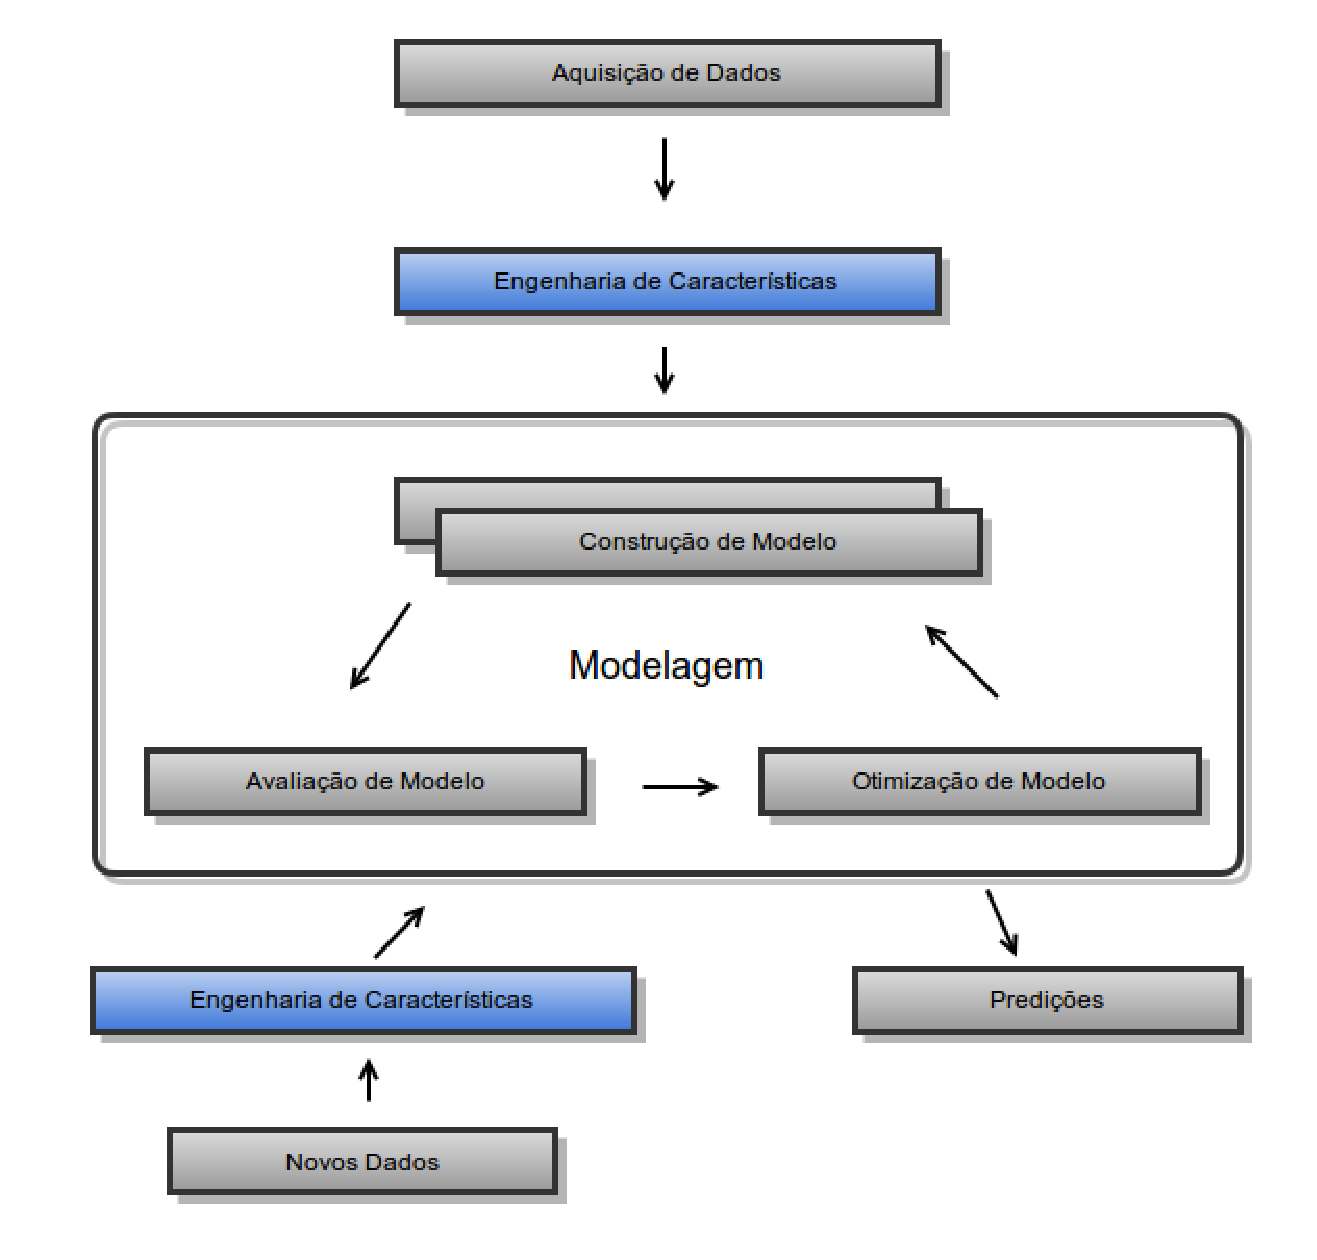
\includegraphics[keepaspectratio=true,scale=0.50]
{figuras/workflowml.eps}
\caption{Workflow de AM}
\label{workflow_am}
\end{figure}

\begin{enumerate}
\item Aquisição dos dados
\item Engenharia de Características
\item Construção do modelo
\item Avaliação do modelo
\item Otimização do modelo
\item Predições
\end{enumerate}

\section{Aquisição dos dados}
Apesar de parecer trivial, definir a aquisição de dados como uma etapa do projeto de AM é extremamente importante e alguns cuidados especiais devem ser considerados para que as predições tenham um bom desempenho. O primeiro passo antes de começar o projeto de AM é saber qual a necessidade do mundo real que deve ser atendida. Este passo pode ser entendido como a necessidade de encontrar questões que envolvem uma variável de interesse (quem gostaria de comprar este produto, qual o significado deste audio em linguagem natural, onde está a face humana nesta imagem,...) e o caminho pra solução que envolve variáveis independentes (histórico de compras dos usuários, mapeamento de sons para texto, características de faces humanas).

Nem sempre utilizar Aprendizagem de Máquina é a melhor resposta para solucioanar os problemas do mundo real. É nessário avaliar com cuidado quais os objetivos da solução e qual o contexto do problema. Um grande indício de que o problema pode ser solucionado por AM é se ele possui algumas das seguintes características: Alta complexidade de relaciomento entre entradas e saídas, grande volume de dados, necessidade de generalização e necessidade de adaptabilidade a novos cenários. 

Os dados que servem como entrada para os processos de modelagem geralmente estão apresentados na forma de tabelas que possuem colunas e linhas. As colunas representam as características dos dados, como se fossem meta-dados, e as linhas representam instâncias dessas características. A tabela a seguir representa os tipos de dados que podem aparecer como característica de dados na Aprendizagem de Máquina \cite{guy2010}.

\begin{table}[h]
\centering
\caption{Tipos de Dados}
\vspace{0.5cm}
\begin{tabular}{r|lr}

\hline 
Tipo & Exemplo  \\ % Note a separação de col. e a quebra de linhas
\hline                               % para uma linha horizontal
Átomo Categórico        & Uma palavra na língua portuguesa \\
\hline   
Átomo Numérico & Valor de temperatura \\
\hline 
Átomo Ordinário           & Preferência cinematográfica (Número de Estrelas) \\
\hline 
Conjunto desordenado de números       & Sinais vitais(pulso, temperatura, pressão sanguínea)\\
\hline 
Conjunto desordenado de misturas     & Informação demográfica(raça, sexo, idade, renda)\\
\hline 
Sequência unidimensional de categóricos       & Documento de texto\\
\hline 
Sequência unidimensional de números       & Série Temporal Financeira\\
\hline 
Sequência bidimensional de números      & Imagem\\
\hline 
Sequência tridimensional de números       & Filme\\
\hline 
Grafo Arbitrário Categórico       & Árvore de Conversões\\
 \hline 
\end{tabular}
\end{table}

A figura a seguir é uma pequena seleção da base de dados que contém informações sobre os passageiros que estavam presentes no naufrágio do Titanic \cite{titanic2012}. 

\begin{figure}[!h]
\centering
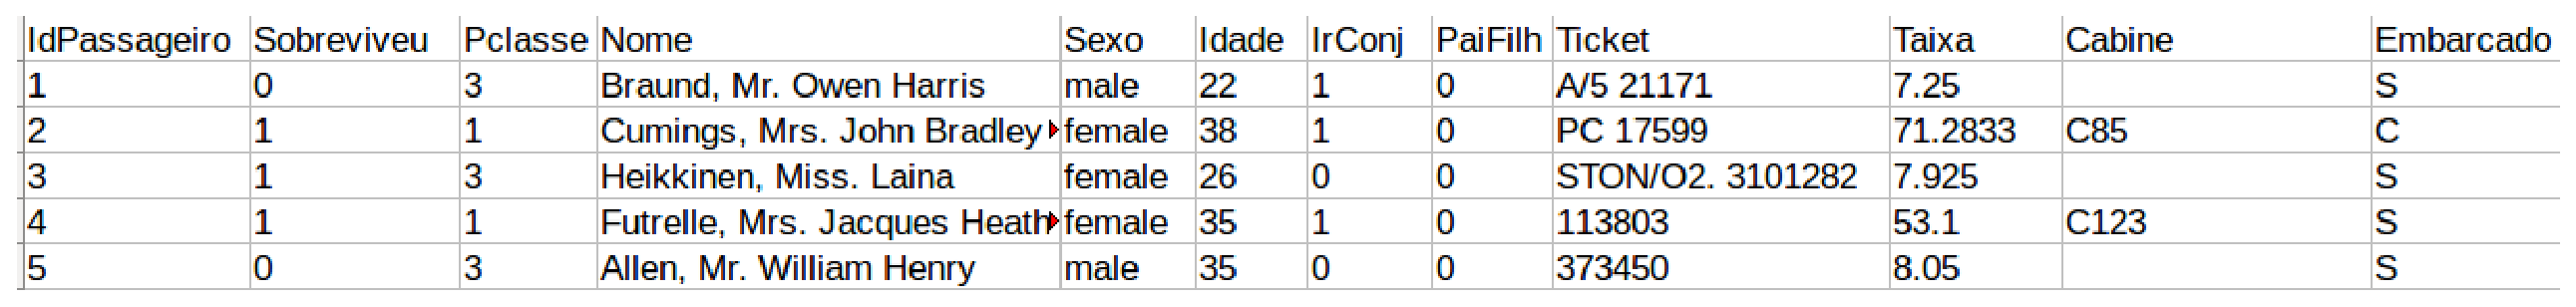
\includegraphics[keepaspectratio=true,scale=0.50]
{figuras/dataEg.eps}
\caption{Exemplo de Dados do Titanic}
\label{data_titatic}
\end{figure}

Cada linha corresponde as informações de um passageiro e cada coluna representa um tipo de informação deste passageiro. A enumeração a seguir explica o que cada linha significa.

\begin{enumerate}
\item IDPassageiro: Um átomo numérico que identifica unicamente cada passageiro.
\item Sobreviveu: Um átomo númerico que representa se a pessoa sobreviveu ou não ao naufráfio. Assume valor "1" para sobreviventes e "0" para não sobreviventes.
\item Pclasse: Átomo numérico que varia de "1" a "3", representa a classe do passageiro. "1" equivale a primeira classe, "2" a segunda classe e "3" a terceira.
\item Nome: Átomo categórico que representa o nome do passageiro.
\item Sexo: Átomo categórico que representa o sexo do passageiro.
\item Idade: Átomo numérico que representa a idade do passageiro.
\item IrConj: Átomo numérico que representa a soma da quantidade de irmãos e cônjuges do passageiro a bordo.
\item PaiFilh: Átomo numérico que representa a soma da quantidade de pais e filhos do passageiro a bordo.
\item Ticket: Átomo categórico que representa o número do ticket de embarque do passageiro.
\item Taixa: Átomo numérico que representa o preço da passagem paga pelo passageiro.
\item Cabine: Átomo categórico que representa o número da cabine do passageiro.
\item Embarcado: Átomo categórico que representa o porto de emabarque do passageiro. "C"  para a cidade de Cherbourg, "Q"  para a cidade de Queesntown e "S"  para Southhampton.

\end{enumerate}


\section{Engenharia de Características}
\section{Construção do modelo}
\section{Avaliação do modelo}
\section{Otimização do modelo}
\section{Predições}





Contexto de ML
Justificativa (Número, Big Data, Aprendizado incremental)
Processos de ML (Tipos de pré-processamento)

